\chapter{Predikcia sekundárnej štruktúry}

Na zlepšenie rýchlosti a presnosti predikovania nekonzervovaných úsekov sme ako prvé opatrenie navrhli riešiť najprv jednoduchší problém, a to predikciu sekundárnej štruktúry targetu, a pomocou nej neskôr predikovať terciárnu štruktúru nekonzervovaných úsekov, čo nás vedie k predpokladu, že by sa mohol výrazne zmenšiť prehľadávaný priestor pri generovaní kandidátskych štruktúr algoritmom FARFAR. Principiálne teda najprv komparatívnym modelovaním napredikujeme sekundárnu target štruktúru, a tú potom poskytneme ako vstup algoritmu FARFAR, ktorý ju použije pri predikcii terciárnej target štruktúry. Tento postup a jeho výsledky sme popísali aj v článku \cite{8218009}.

\section{Príprava dát}
Pretože algoritmus doplníme o komparatívne predikovanie sekundárnej štruktúry, nebude na vstupe potrebovať len sekvenciu target molekuly a sekvencie terciárnej štruktúry template molekuly, ale aj sekundárnu štruktúru template molekuly. Štruktúru očakávame v dot-bracket notácii. Sekundárnu štruktúru by bolo možné získať z terciárnej aj počas predikcie, avšak v prípade, kedy si užívateľ chce dodať inú sekundárnu štruktúru, je preňho výhodnejšie, keď je sekundárna štruktúra dodaná ako ďalší vstupný parameter.


\indent Získať dáta sme sa rozhodli ich určením z terciárnej štruktúry programom DSSR (Defining the Secondary Structures of RNA) zo software balíku x3DNA \cite{x3dna}. Na hromadné extrahovanie štruktúr sme si potom vytvorili dva krátke scripty, ktoré sa nachádzajú v \url{MyTools/PredictSecondaryStructures/}. DSSR vytvára v sekundárnej štruktúre base-pairs vyznačené jednoduchými zátvorkami, ako aj pseudo uzly vyznačené hranatými zátvorkami \ref{obr5.0}. Z dôvodov implementačných komplikácií a zladenia s algoritmom FARFAR sme sa rozhodli pracovať iba so sekundárnou štruktúrou označujúcou base-pairs, a preto pseudo uzly neberieme do úvahy.
\begin{figure}%[p]\centering
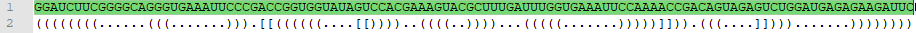
\includegraphics[width=\textwidth]{../img/dssr}
\caption{Príklad súboru sekundárnej štruktúry získanej progrmaom DSSR zo štruktúry terciárnej. V prvom riadku sú príslušné typu nukleotidov a v druhom riadku je samotná sekundárna štruktúra v  dot-bracket reprezentácii.}
\label{obr5.0}
\end{figure}


\section{Predikcia sekundárnej štruktúry}
Sekundárnu štruktúru predikujeme rovnakým spôsobom ako štruktúru terciárnu, teda komparatívnym modelovaním. Ako vstup potrebuje algoritmus dostať sekvenciu target molekuly a sekvenciu aj sekundárnu štruktúru template molekuly. 


\indent  Používame rovnakú template štruktúru ako pre terciárnu predikciu, a preto sa algoritmus predikcie sekundárnej štruktúry zhoduje s algoritmom predikcie terciárnej štruktury až po získanie konzervovaných úsekov v zarovnaní \ref{3-indels}. Následne potrebujeme na zarovnanie namapovať sekundárnu template štruktúru. Tu musíme riešiť nasledujúcu situáciu: ak práve jeden nukleotid z base-pair nie je konzervovaný a druhý konzervovaný je, musíme v sekundárnej štruktúre preznačiť oba nukleotidy ako nespárované. Tiež to môžeme chápať tak, že sekundárnu štruktúru udržujeme stále správne uzátvorkovanú, čo znamená, že zátvorky rovnakého typu sa navzájom nekrížia, a teda máme rovnaký počet pravých aj ľavých zátvoriek v sekundárnej štruktúre.


\indent Namapovaním sekundárnej štruktúry na alignment získame neúplnú sekundárnu štruktúru target molekuly. Túto následne predáme spolu s target sekvenciou nástroju RNAfold \cite{RNAfold}, ktorý predikuje sekundárnu štruktúru vzhľadom na obmedzenia plynúce z dodanej sekundárnej štruktúry. Dĺžka predikcie sa pohybuje v rádoch jednotiek až desiatok sekúnd, takže to nepredstavuje židne citeľné spomalenie celého algoritmu. 


\section{Integrácia do existujúceho algoritmu}
Do konfiguračného súboru sme pridali nastavenie, ktoré určuje, či algoritmus pracuje aj so sekundárnou štruktúrou, alebo nie.


\indent Z pohľadu začlenenia do algoritmu sa sekundárna štruktúra predikuje krokom \ref{3-map} mapujúcim terciárnu template štruktúru na alignment. V ďalšom kroku, ktorý ošetruje dlhé medzery, už namapovanú sekundárnu štruktúru používame na to, aby sme k fragmentom terciárnej štruktúry slúžiacej ako template pre FARFAR vybrali aj fragmenty sekundárnej štruktúry. Keďže FARFAR-u musíme dať validnú sekundárnu štruktúru v dot-bracket notácii, v prípade, ak je do predikcie dlhého nekonzervovaného úseku vybraný z base-pairu v sekundárnej štruktúre práve jeden nukleotid, musíme pridať aj druhý, aby sme zachovali validitu sekundárnej štruktúry. To isté musíme riešiť v ďalšom kroku, keď pripravujeme predikciu zvyšku štruktúry už bez dlhých nekonzervovaných úsekov. 


\indent Nakoniec bolo treba upraviť shell scripty tak, aby nakopírovali na správne miesta súbory so sekundárnymi štruktúrami, a v parametri predať príslušný template súbor so sekundárnou štruktúrou algoritmu FARFAR.

\section{Experiment a Výsledky}
Za účelom overenia vplyvu pridania predikcie sekundárnej štruktury do pôvodného algoritmu sme urobili rovnaké testovanie nad rovnakými dátami, ako pri porovnávaní pôvodného algoritmu s ModeRNA. Skúšali sme napredikovať všetky páry s podobnosťou medzi 60\% - 90\% a dĺžkou 50-100 a 101-500 nukleotidov najprv pôvodnou verziou algoritmu Trooper, verziou algoritmu vylepšenou o predikciu sekundárnej štruktúry a referenčnou predikciou ModeRNA. 


\indent  Výsledky a porovnanie predikcií uvádzame v tabuľke \ref{tab5.1}. Z výsledkov vidíme, že pridanie predikcie sekundárnej štruktúry spôsobilo, že priemerná RMSD pre štruktúry s dĺžkou medzi 50-100 nukleotidov a 413 úspešne napredikovaných pároch sa zhoršila z 5,80Å na 8,23Å, čo približne zodpovedá výsledku 8,53Å, ktoré na predikcii rovnakých štruktúr dosiahla ModeRNA. Pri predikcii štruktúr dĺžky 101-500 nukleotidov a 98 úspešne napredikovaných pároch sa naopak priemerné výsledky predikcie s pridaním predikcie sekundárnej štruktýry výrazne zlepšili a to z 6,91Å na 3,46Å, čo je o niečo lepšie než výsledky ModeRNA, ktorá pri rovnakých podmienkach dosiahla priemer 3,72Å. 
\begin{table}[b!]
\centering
\begin{tabular}{ccccc}
\toprule
Veľkosť & Počet párov & Trooper bez SS & Trooper s SS & ModeRNA\\
\midrule
50-100  & 413 & 5,80  & 8,23 & 8,53\\
101-500  & 98 & 6,91  & 3,46 & 3,72\\
\bottomrule
50-500  &  511 & 5,95  & 7,31 & 7,61\\
\end{tabular}
\caption{Porovnanie priemernej RMSD predikcie RNA nástrojmi Trooper, Trooper s predikciou sekundárnej štruktúry a ModeRNA. }\label{tab5.1}
\end{table}


\indent Z výsledkov je teda zrejmé, že pridanie predikcie sekundárnej štruktúry a jej poskytnutie algoritmu FARFAR v niektorých prípadoch výsledky zlepšilo a v niektorých zhoršilo. Prečo boli zlepšené práve dlhšie štruktúry by sme mohli vysvetliť tak, že dlhšie štruktúry môžu obsahovať dlhšie nekonzervované úseky, ktorých predikcia je pre FARFAR náročnejšia. Príklad z obrázka \ref{obr5.1} práve podporuje takúto teóriu, kedy vidíme, že pôvodná predikcia FARFAR bez sekundárnej štruktúry napredikovala nekonzervovaný úsek zle, ale po pridaní sekundárnej štruktúry sa FARFAR-u podarilo úsek napredikovať oveľa presnejšie.
\begin{figure}%[p]\centering
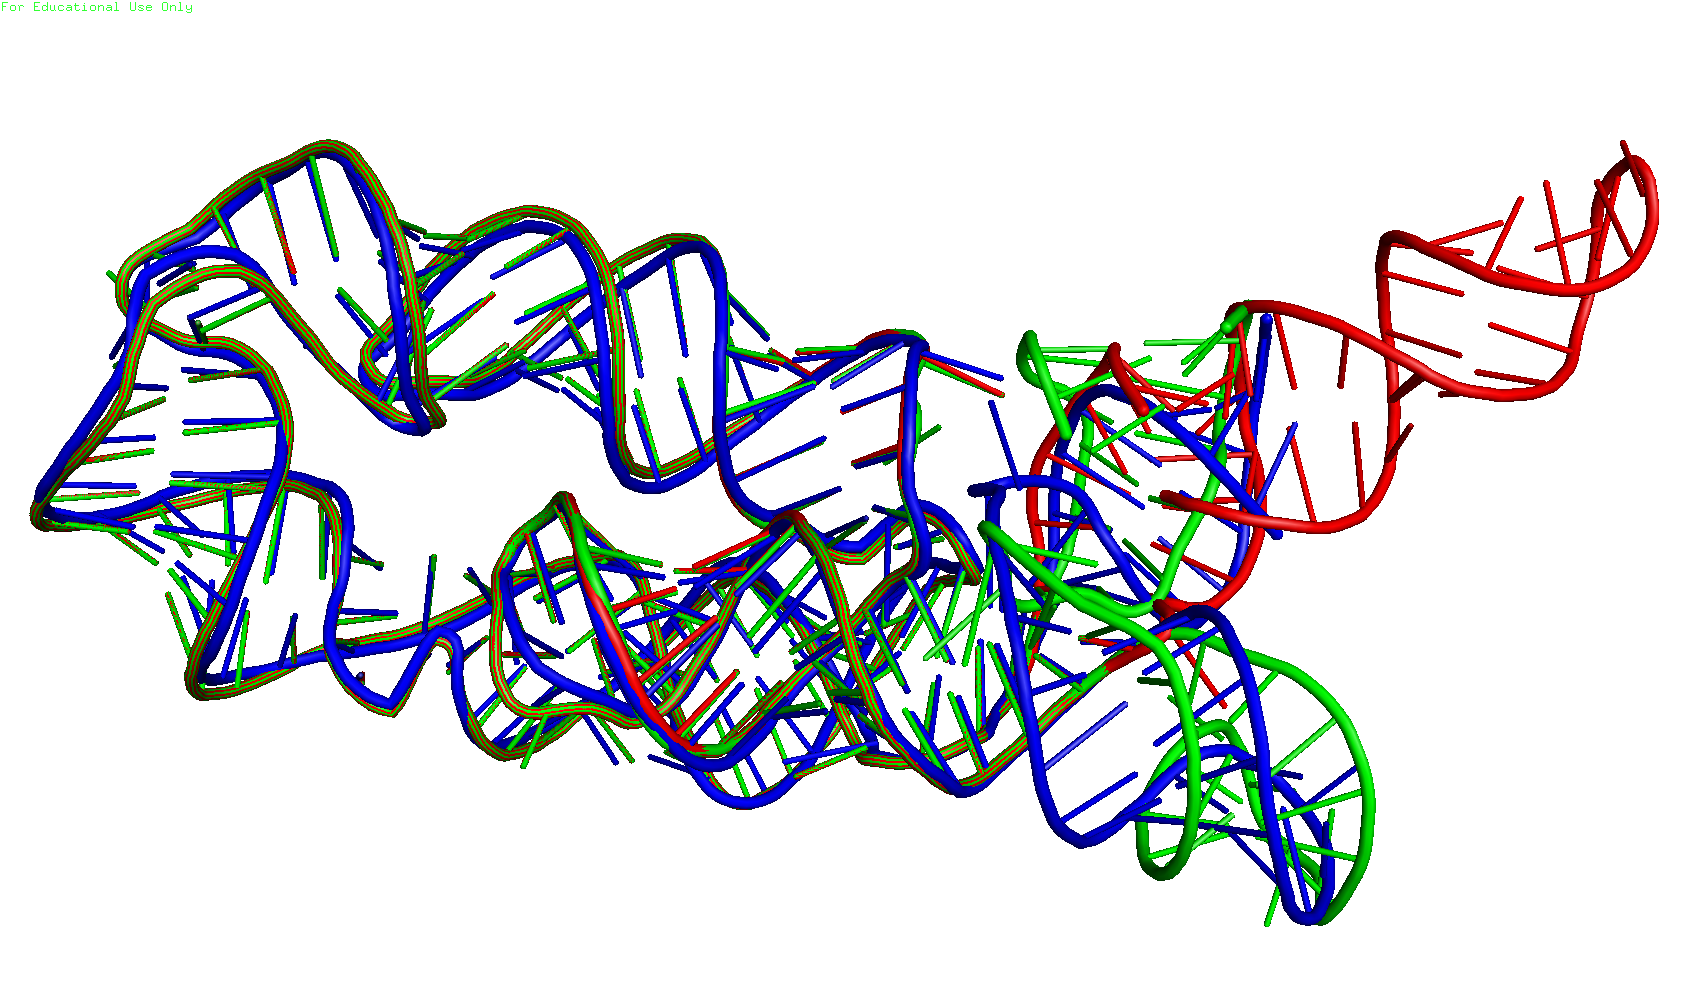
\includegraphics[width=\textwidth]{../img/struct1}
\caption{Modrá štruktúra je experimentálne získana štruktúra molekuly 3DIG:X s dĺžkou 175 nukleotidov. Červená štruktúra je predikovaná algoritmom Trooper bez použitia sekundárnej štruktúry s výslednou RMSD na úrovni 14,44Å. Zelená štruktúra je predikcia urobená algoritmom Trooper s výslednou RMSD 4,44Å. Pre obe predikcie bol použitý rovnaký template, a to štruktúra 3DOU:A.}
\label{obr5.1}
\end{figure}


\indent Ďalej sme ešte skúmali značné zhoršenie výsledkov v triede štruktúr veľkostí 50-100 nukleotidov z RMSD 5,8Å na 8,23Å. Zastávame hypotézu, že by to mohlo byť spôsobené nesprávnou sekundárnou štruktúrou dodanou algoritmu FARFAR, pretože inak boli podmienky oboch predikcií rovnaké, a teda by sa priemerné výsledky nemali od seba značne líšiť.


\indent Správnosť predikovanej sekundárnej štruktúry vieme popísať a klasifikovať štyrma mierami: true positives (správne určený existujúci base-pair), true negatives (správne určený nespárovaný nukleotid), false positives (nesprávne určený base-pair) a nakoniec false negative (v štruktúre by mal existovať base-pair, ale nie je napredikovaný). Z týchto štyroch ukazateľov sú prvé dva pozitívne a druhé dva negatívne. Pritom ale FARFAR-u môže uškodiť iba prípad false negative, pretože ten mu indikuje, že má v predikcii spárovať (a teda umiestniť blízko seba) dva nukleotidy. Prípady s false negatives by predikciu FARFAR-u nemali zlepšiť, ale ani zhoršiť, pretože nekladú žiadnu podmienku na spárovanie nukleotidov. 


\indent Zamerali sme sa preto na prípady false positives v predikovaných sekundárnych štruktúrach a analyzovali sme koreláciu medzi zhoršením, prípadne zlepšením predikcie algoritmu Trooper bez sekundárnej štruktúry a algoritmu Trooper s predikciou sekundárnej štruktúry vzhľadom na počet false positives v napredikovanej sekundárnej štruktúre dodanej ako vstup algoritmu FARFAR. Výsledok je graficky znázornený na obrázku \ref{obr5.2} a podporuje našu hypotézu o tom, že čím viac vzrastal počet false positives v predikovanej sekundárnej štruktúre, tým bolo pravdepodobnejšie, že predikcia so sekundárnou štruktúrou sa oproti predikcii bez sekundárnej štruktúry zhorší. Preto si myslíme, že zhoršenie v niektorých preikciách bolo spôsobené hlavne zle napredikovanou sekundárnou štruktúrou.
\begin{figure}%[p]\centering
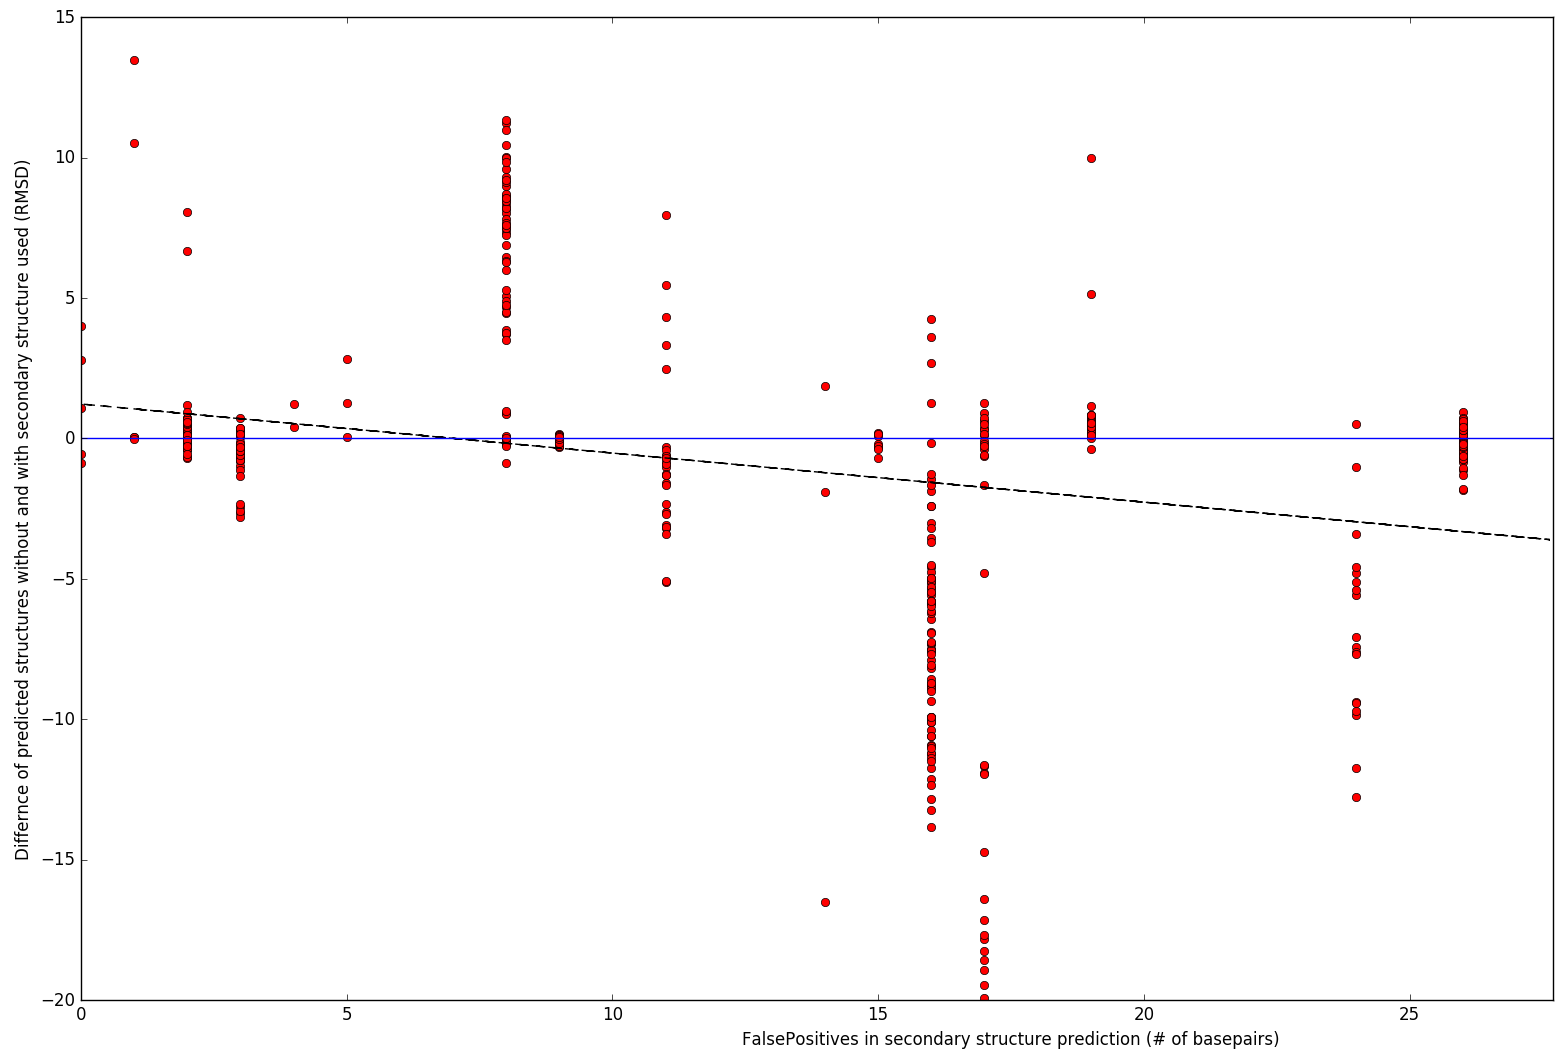
\includegraphics[width=\textwidth]{../img/corelation}
\caption{Závislosť medzi rozdielom výsledkov predikcie s a bez sekundárnej štruktúry a počtom false positive base-pairs v napredikovanej sekundárnej štruktúre. Červené body sú jednotlivé záznamy a čiarkovanou čiarou je zobrazená lineárna regresia týchto bodov.}
\label{obr5.2}
\end{figure}